\documentclass[border=10pt]{standalone}
\usepackage[default]{lato}
\usepackage[T1]{fontenc}
\usepackage{verbatim}
\usepackage{xcolor}
\usepackage{tikz}
\usetikzlibrary{shapes,arrows,arrows.meta,mindmap,backgrounds,calc,positioning}

\tikzset{
	>={Latex[width=2mm,length=2mm]},
	% Specifications for style of nodes:
	base/.style = {rectangle, rounded corners, 
	minimum width=2.5cm, minimum height=1cm,
	draw=black, line width=0.3mm,
	text centered, font=\small},
	l0/.style ={rectangle,
	minimum width=2.5cm, minimum height=2cm,
	draw=gray50, line width=1mm,
	text centered, font=\small},
	l1/.style ={rectangle,
	minimum width=2.5cm, minimum height=2cm,
	draw=darkorange, line width=1mm,
	text centered, font=\small},
	l2/.style ={rectangle,
	minimum width=2.5cm, minimum height=2cm,
	draw=darkorchid, line width=1mm,
	text centered, font=\small},
	l3a/.style ={rectangle,
	minimum width=2.5cm, minimum height=2cm,
	draw=mediumseagreen, line width=1mm,
	text centered, font=\small},
	l3b/.style ={rectangle,
	minimum width=2.5cm, minimum height=2cm,
	draw=dodgerblue, line width=1mm,
	text centered, font=\small},
	ext/.style ={rectangle,
	minimum width=1cm, minimum height=1cm,
	draw=red, line width=1mm,
	text centered, font=\small},
}

\definecolor{darkorange}{RGB}{255,140,0}
\definecolor{mediumseagreen}{RGB}{60, 179, 113}
\definecolor{darkorchid}{RGB}{153, 50, 204}
\definecolor{dodgerblue}{RGB}{30, 144, 255}
\definecolor{gray50}{RGB}{128,128,128}

\begin{document}
\resizebox{\textwidth}{!}{
	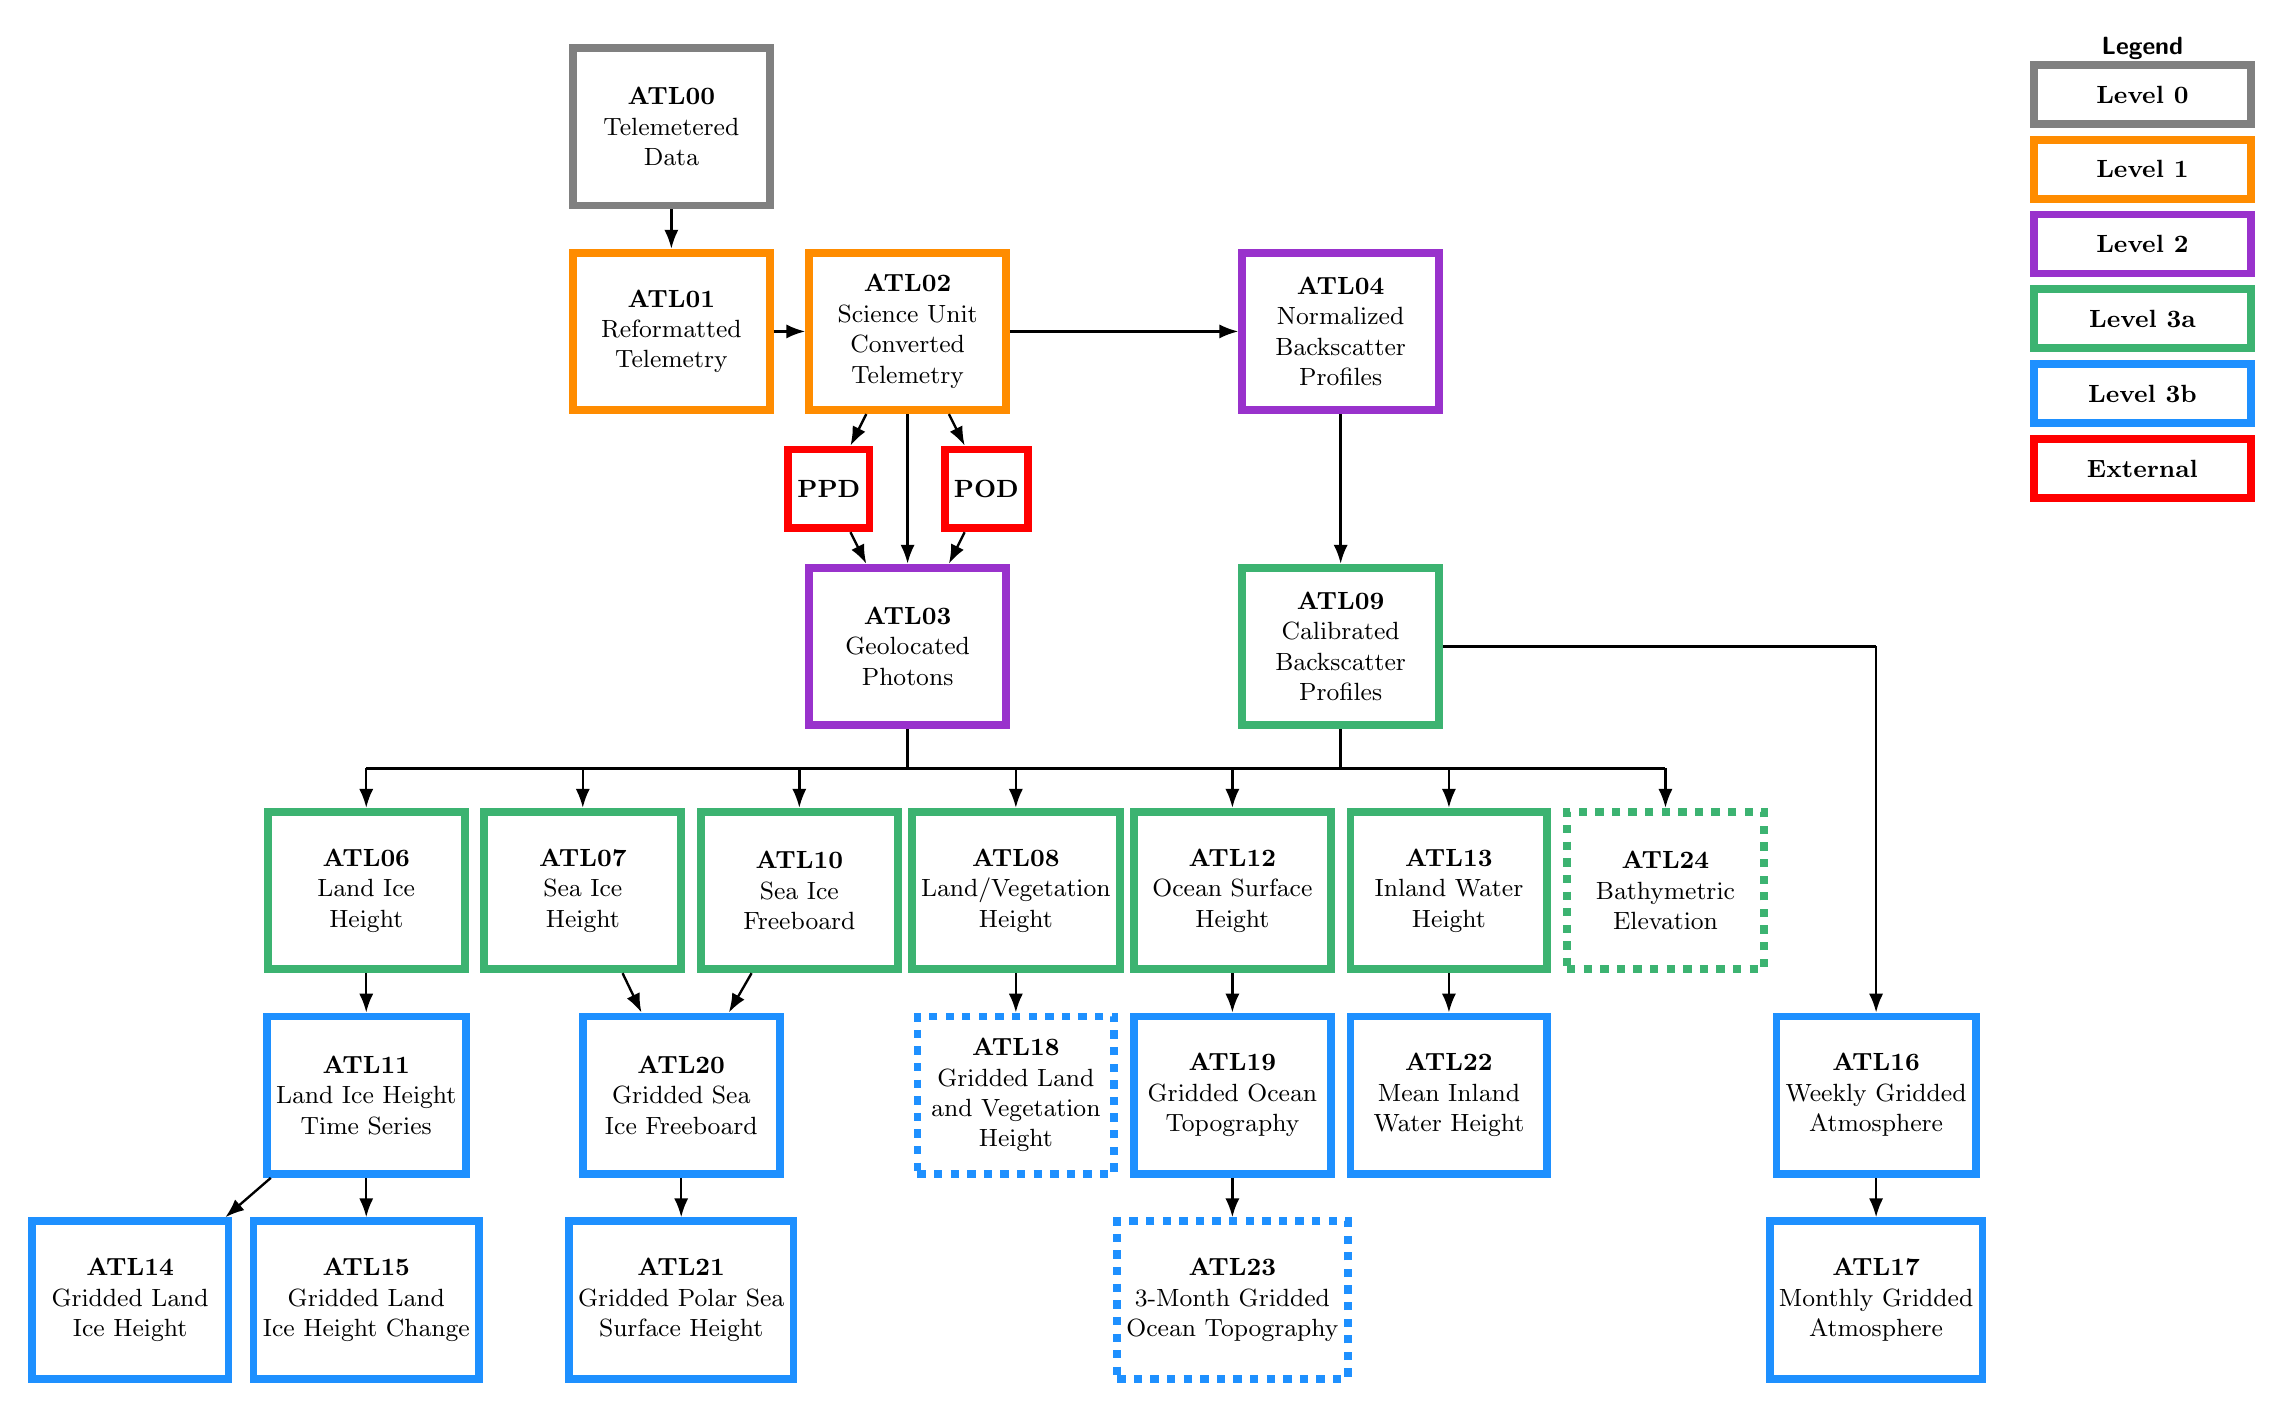
\begin{tikzpicture}[node distance=2cm, every node/.style={fill=white, font=\small\sffamily}, align=center]
	\linespread{1}
		% draw blocks
		\node (atl00)[l0]{\textbf{ATL00}\\Telemetered\\Data};
		\node (atl01)[l1, below=0.5cm of atl00]{\textbf{ATL01}\\Reformatted\\Telemetry};
		\node (atl02)[l1, right of=atl01, xshift=1cm]{\textbf{ATL02}\\Science Unit\\Converted\\Telemetry};
		\node (ppd)[ext, below of=atl02, xshift=-1cm]{\textbf{PPD}};
		\node (pod)[ext, below of=atl02, xshift=1cm]{\textbf{POD}};
		% Level 2 products
		\node (atl03)[l2, below of=ppd, xshift=1cm]{\textbf{ATL03}\\Geolocated\\Photons};
		\node (atl04)[l2, right of=atl02, xshift=3.5cm]{\textbf{ATL04}\\Normalized\\Backscatter\\Profiles};
		% connection coordinates for single arrow out of ATL03
		\node(A)[shape=coordinate, below=0.5cm of atl03] {};
		\node (B)[shape=coordinate, left=1.375cm of A] {};
		\node (C)[shape=coordinate, left=2.75cm of B] {};
		\node (D)[shape=coordinate, left=2.75cm of C] {};
		\node (E)[shape=coordinate, right=1.375cm of A] {};
		\node (F)[shape=coordinate, right=2.75cm of E] {};
		\node (G)[shape=coordinate, right=2.75cm of F] {};
		\node (H)[shape=coordinate, right=2.75cm of G] {};
		% Level 3a products
		\node (atl06)[l3a, below=0.5cm of D]{\textbf{ATL06}\\Land Ice\\Height};
		\node (atl07)[l3a, below=0.5cm of C]{\textbf{ATL07}\\Sea Ice\\Height};
		\node (atl10)[l3a, below=0.5cm of B]{\textbf{ATL10}\\Sea Ice\\Freeboard};
		\node (atl08)[l3a, below=0.5cm of E]{\textbf{ATL08}\\Land/Vegetation\\Height};
		\node (atl12)[l3a, below=0.5cm of F]{\textbf{ATL12}\\Ocean Surface\\Height};
		\node (atl13)[l3a, below=0.5cm of G]{\textbf{ATL13}\\Inland Water\\Height};
		\node (atl24)[l3a, dashed, below=0.5cm of H]{\textbf{ATL24}\\Bathymetric\\Elevation};
		\node (atl09)[l3a, right of=atl03, xshift=3.5cm]{\textbf{ATL09}\\Calibrated\\Backscatter\\Profiles};
		% connection coordinates for single arrow out of ATL09
		\node (I)[shape=coordinate, below=0.5cm of atl09] {};
		\node (J)[shape=coordinate, right=5.5cm of atl09] {};
		% Level 3b products
		\node (atl11)[l3b, below=0.5cm of atl06]{\textbf{ATL11}\\Land Ice Height\\Time Series};
		\node (atl14)[l3b, below=0.5cm of atl11, xshift=-3cm]{\textbf{ATL14}\\Gridded Land\\ Ice Height};
		\node (atl15)[l3b, below=0.5cm of atl11, xshift=0cm]{\textbf{ATL15}\\Gridded Land\\ Ice Height Change};
		\node (atl20)[l3b, below=0.5cm of atl10, xshift=-1.5cm]{\textbf{ATL20}\\Gridded Sea\\ Ice Freeboard};
		\node (atl21)[l3b, below=0.5cm of atl20, xshift=0cm]{\textbf{ATL21}\\Gridded Polar Sea\\ Surface Height};
		\node (atl18)[l3b, dashed, below=0.5cm of atl08, xshift=0cm]{\textbf{ATL18}\\Gridded Land\\ and Vegetation\\Height};
		\node (atl19)[l3b, below=0.5cm of atl12]{\textbf{ATL19}\\Gridded Ocean\\Topography};
		\node (atl23)[l3b, dashed, below=0.5cm of atl19]{\textbf{ATL23}\\3-Month Gridded\\Ocean Topography};
		\node (atl22)[l3b, below=0.5cm of atl13]{\textbf{ATL22}\\Mean Inland\\Water Height};
		\node (atl16)[l3b, below=4.65cm of J]{\textbf{ATL16}\\Weekly Gridded\\Atmosphere};
		\node (atl17)[l3b, below=0.5cm of atl16]{\textbf{ATL17}\\Monthly Gridded\\Atmosphere};
		% Legend
		\node (legend)[right=16cm of atl00, yshift=1cm, minimum height=0cm, minimum width=2.75cm]{\textbf{Legend}};
		\node (level0)[l0, below=-0.1cm of legend, minimum height=0.75cm, minimum width=2.75cm]{\textbf{Level 0}};
		\node (level1)[l1, below=0.1cm of level0, minimum height=0.75cm, minimum width=2.75cm]{\textbf{Level 1}};
		\node (level2)[l2, below=0.1cm of level1, minimum height=0.75cm, minimum width=2.75cm]{\textbf{Level 2}};
		\node (level3a)[l3a, below=0.1cm of level2, minimum height=0.75cm, minimum width=2.75cm]{\textbf{Level 3a}};
		\node (level3b)[l3b, below=0.1cm of level3a, minimum height=0.75cm, minimum width=2.75cm]{\textbf{Level 3b}};
		\node (extern)[ext, below=0.1cm of level3b, minimum height=0.75cm, minimum width=2.75cm]{\textbf{External}};
		% draw arrows between nodes
		\draw[line width=0.3mm,-Latex](atl00) -- (atl01);
		\draw[line width=0.3mm,-Latex](atl01) -- (atl02);
		\draw[line width=0.3mm,-Latex](atl02) -- (ppd);
		\draw[line width=0.3mm,-Latex](atl02) -- (pod);
		\draw[line width=0.3mm,-Latex](ppd) -- (atl03);
		\draw[line width=0.3mm,-Latex](pod) -- (atl03);
		\draw[line width=0.3mm,-Latex](atl02) -- (atl03);
		\draw[line width=0.3mm,-Latex](atl02) -- (atl04);
		\draw[line width=0.3mm,-Latex](atl04) -- (atl09);
		\draw[line width=0.3mm,-](atl03.south) -- (A.north);
		\draw[line width=0.3mm,-](atl09.south) -- (I.north);
		\draw[line width=0.3mm,-](atl09.east) -- (J.west);
		\draw[line width=0.3mm,-](A.west) -- (D.east);
		\draw[line width=0.3mm,-](A.east) -- (H.west);
		\draw[line width=0.3mm,-Latex](D.south) -- (atl06.north);
		\draw[line width=0.3mm,-Latex](C.south) -- (atl07.north);
		\draw[line width=0.3mm,-Latex](B.south) -- (atl10.north);
		\draw[line width=0.3mm,-Latex](E.south) -- (atl08.north);
		\draw[line width=0.3mm,-Latex](F.south) -- (atl12.north);
		\draw[line width=0.3mm,-Latex](G.south) -- (atl13.north);
		\draw[line width=0.3mm,-Latex](H.south) -- (atl24.north);
		\draw[line width=0.3mm,-Latex](J.south) -- (atl16.north);
		\draw[line width=0.3mm,-Latex](atl06) -- (atl11);
		\draw[line width=0.3mm,-Latex](atl11) -- (atl14);
		\draw[line width=0.3mm,-Latex](atl11) -- (atl15);
		\draw[line width=0.3mm,-Latex](atl07) -- (atl20);
		\draw[line width=0.3mm,-Latex](atl10) -- (atl20);
		\draw[line width=0.3mm,-Latex](atl20) -- (atl21);
		\draw[line width=0.3mm,-Latex](atl08) -- (atl18);
		\draw[line width=0.3mm,-Latex](atl12) -- (atl19);
		\draw[line width=0.3mm,-Latex](atl19) -- (atl23);
		\draw[line width=0.3mm,-Latex](atl13) -- (atl22);
		\draw[line width=0.3mm,-Latex](atl16) -- (atl17);
	\end{tikzpicture}
}
\end{document}
%%% Local Variables: ***
%%% mode: latex ***
%%% TeX-master: "ASAS_product_chart.tex" ***
%%% End: ***
